\section{From Policies to Paths} \label{sec:architecture}
Directly generating policy-compliant configurations is a challenging
problem.
Therefore, all the techniques we present in this paper 
use a two-phased approach in which we first synthesize
policy-compliant \emph{paths} using the tool \genesis~\cite{genesis}
and then use the synthesized paths as \emph{hints} to synthesize resilient configurations. 
In this section, we recall the features of \genesis,
 a tool for generating policy-compliant paths, and describe
some modifications that are necessary to generate paths that
can be realized by routing protocols. 

%that result in the paths we
%synthesized in the first phase; we refer to tool that performs the second phase as \name.
%The first phase may produce \emph{bad} paths for which the
%configuration synthesis is complicated or not possible. Thus, we
%propose ways to restart the algorithm by computing new paths.

%\subsection{\genesis: From Policies to Paths} \label{sec:genesis}
\genesis~\cite{genesis} is a network management
system which synthesizes forwarding tables enforcing some input policies. 
Some of the policies supported by \genesis are specified in 
\Cref{tab:policysupport}. 
%Due to the rich policy language, generating policy-compliant paths is an NP-complete problem;
%\genesis mitigates this problem by leveraging the power of SMT solvers.
% to provide
%support for policy enforcement for a diverse set of policies.
Given a set of policies, \genesis generates a set of constraints 
over propositional logic (SAT) and Linear rational arithmetic (LRA);
the solutions to these constraints are forwarding
tables, which can be used to extract the 
policy-compliant paths.

\genesis uses the relation $Fwd \subseteq V \times V \times PC $  
to capture 
the network forwarding behavior---i.e. 
$(r_1, r_2$, $pc)\in$ $Fwd$ if 
$r_1$ forwards packets of class $pc$ to router $r_2$---
and 
the relation $Reach \subseteq V \times PC \times \nat$ 
to capture
 path reachability---i.e. $(r, pc, k)\in Reach$ if 
the router $r$ is reachable in the path from the source
router of packet class $pc$ in exactly $k$ steps. Based on
the input policies, \genesis generates constraints over the $Fwd$
and $Reach$ relations. Finally, \genesis uses the solution to the relations to extracts the concrete paths.
\begin{figure}
	\centering
	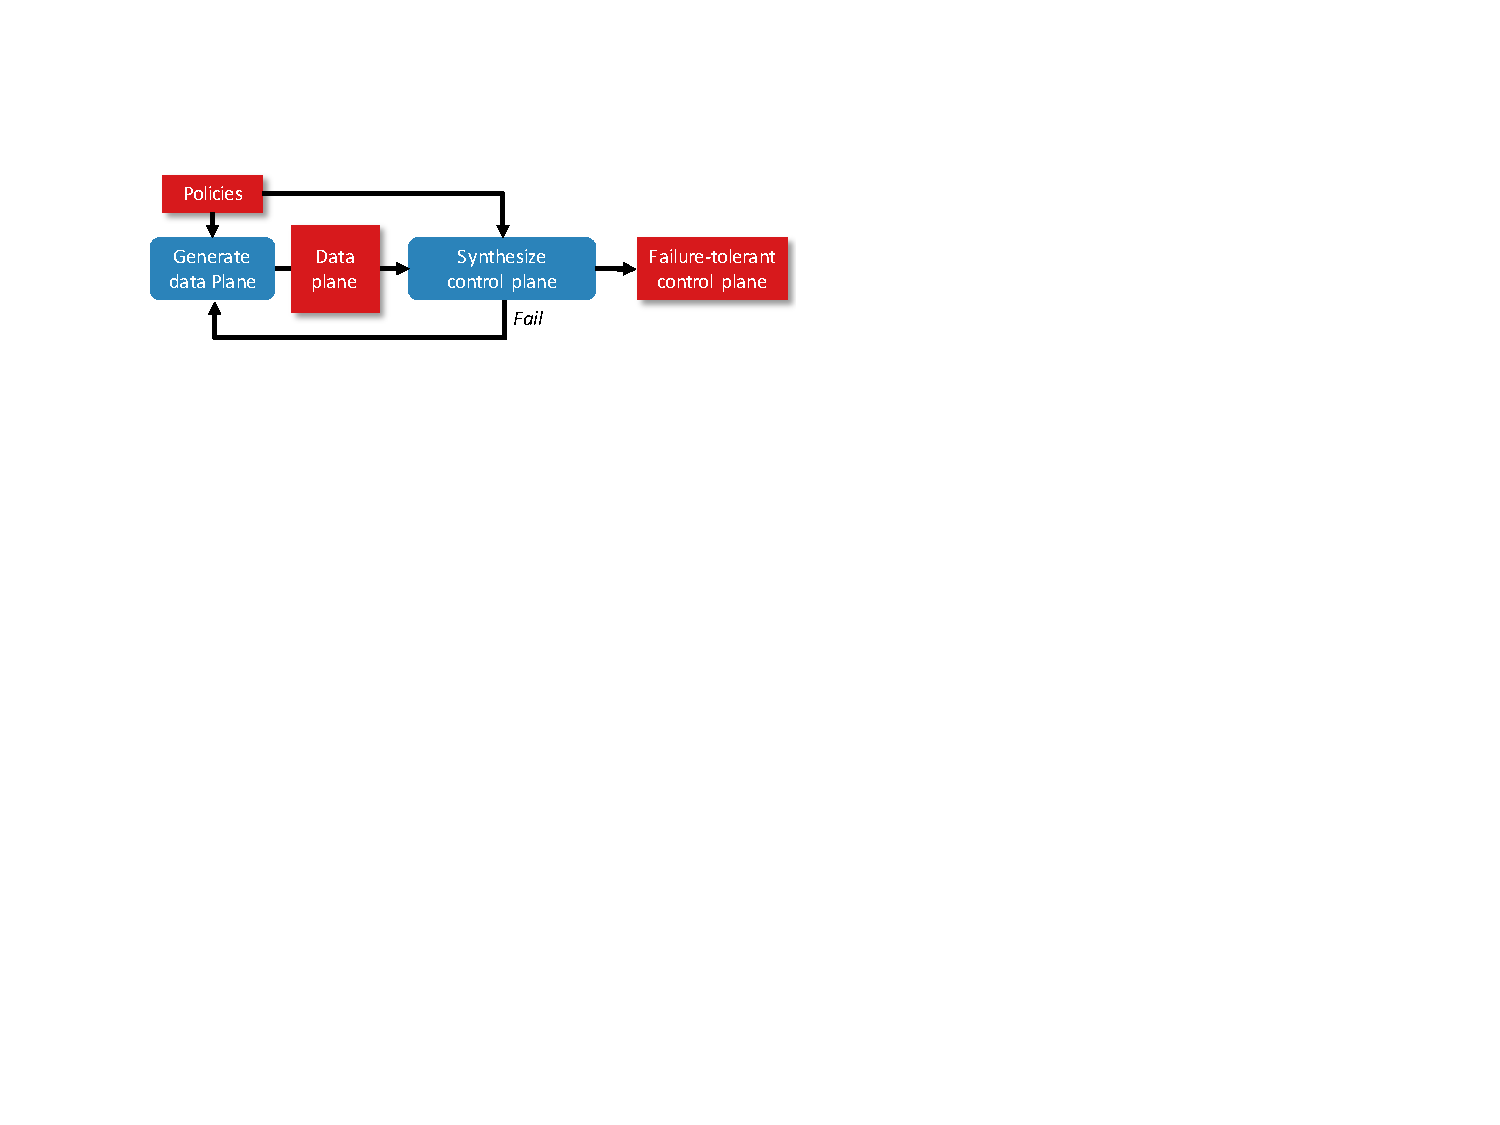
\includegraphics[width=0.5\columnwidth]{figures/architecture.pdf}
	\compactcaption{Two-phase process for generating a control plane
		with failure-tolerance properties}
	\label{fig:architecture}
\end{figure}
\paragraph{Modifications to \genesis}
OpenFlow switches~\cite{openflow} support match predicates for
forwarding rules on different packet header fields such as source
and/or destination IP address, ports etc. However, legacy protocols
like OSPF and BGP only support destination-based forwarding, 
forcing the paths to a destination subnet to 
form a directed tree rooted at the destination. 
Thus,
at any router, there exists at most one forwarding rule per destination. 
Since \genesis was built for
SDN management,  a switch may forward to different switches
packets that are directed to the same destination;
this behaviour cannot be induced by any router
configuration. We  discuss how the
constraints of \genesis~\cite{genesis}
need to be modified to avoid generating paths that 
cannot be enforced by any routing configuration.

Concretely, we modify the constraints given to \genesis to ensure that,
if any two paths to a destination subnet intersect at a router,
the subsequent downstream paths to the destination from the
router do not \emph{diverge} at another router.  
We define the relation $Reach^*(r,pc)$ to model reachability 
of $r$ in the path of $pc$---i.e., $r$ is traversed by the path for packet class $pc$. 
If we allow paths of length at most $\mu$, we can define $Reach^*(r,pc)$ as:
\begin{equation}
	Reach^*(r,pc) \Leftrightarrow \bigvee_{k \in [0, \mu]} Reach(r, pc, k).
\end{equation}
To guarantee that the generate paths can be enforced using destination-based
forwarding we add
the following constraint for every pair of packet classes $pc_1$ and $pc_2$ that belong to the same 
 destination subnet:
 \begin{equation}
 \forall r. Reach^*(r, pc_1) \wedge Reach^*(r, pc_2) 
 \implies \\ \bigwedge_{n \in N(r)} Fwd(r, n, pc_1) \Leftrightarrow Fwd(r, n, pc_2)
 \end{equation}
Intuitively, 
 if a router $r$ is reachable for both packet classes, 
 then the next router $n$ in the path must be the same for both classes
 (paths will not diverge). Thus, the paths obtained
 from \genesis for a destination will form a 
 directed destination tree.
 We will use this property in Section~\ref{sec:intra-synthesis}. 

%\subsection{\name: From Paths to Router Configurations} 
%After we have computed a set of policy-compliant paths,
%we need to solve the path-compliance problem using such paths.
%To solve this problem \name
%combines techniques in constraint solving and randomized search
%to efficiently generate router configurations for the paths obtained from \genesis.
%For a given domain division of the network,
%\name uses linear constraints to generate OSPF weights and 
%the structure of the paths  to generate BGP preferences.
%If the generated linear  constraints cannot be solved, \name uses the unsatisfiable cores to
%identify where to place route filters.
%To decide how to split the network into domains,
%\name uses Markov Chain Monte Carlo (MCMC) search to find
%domain assignments that satisfy the configuration policies and have good resilience.
%When the MCMC search does not progress and cannot find good solutions,
%we restart the search by asking \genesis to generate a new set of paths that is different from
%the previously generated ones.
%These techniques are described in detail in the next two sections.

%\subsection{Challenges}
%\minisection{OSPF Synthesis}
%For the OSPF protocol, configurations assign
%weights to links between routers (directed edges
%in the network topology). When the network has
%to forward a packet from $s$ to $t$, the
%OSPF routers uses 
%Djikstra's algorithm to chose the
%shortest weighted path from $s$ to $t$. Thus,
%given input paths, \name finds edge weights 
%(which are global for all paths) such that 
%the shortest path through the network
%for these endpoints exactly match the input paths. 
%For example in \Cref{fig:ospfexample}(a), if the input
%path is $s\rightarrow r_1 \rightarrow t$ for
%destination IP $\lambda$, \name assigns
%edge weights such that the input path has a strictly
%smaller weight ($w=1+2$) than the other path $s \rightarrow t$ 
%($w=5$). Thus, the OSPF routers will forward traffic for
%$\lambda$ from $s$ to $t$ through $r_1$. \name 
%efficiently computes weights by generating constraints
%in the theory of Linear rational arithmetic (LRA) and
%uses fast off-the-shelf LP Solvers 
%(\secref{sec:ospfsynthesis}). 
%
%However, given a set of paths as input, there may
%not exist a solution to the edge weights. Consider the 
%input paths as shown in \Cref{fig:ospfexample}(b). 
%Both the red and blue paths are required 
%to be the unique shortest path between $s$ to $t$
%and, clearly, this is cannot be enforced for any 
%choice of the edge weights (as weights correspond 
%to all destinations). 
%One way to synthesize configurations in this scenario 
%is to ``disable'' the edge
%$(s, t)$ for destination $\lambda_1$.
%Using this technique, 
%there is only one possible path from $s$ to $t$
%for destination $\lambda_1$ ($s\rightarrow r_1 \rightarrow t$),
%therefore is chosen as the shortest path. For 
%destination $\lambda_2$, the $s\rightarrow t$ path
%has a smaller weight ($w=1$) than the
%$s\rightarrow r_1 \rightarrow t$ path ($w=1+2$), therefore,
%both traffic is forwarded through the input paths for
%both the destinations. 
%This blocking mechanism is called a route filter, and
%we modify \name's OSPF synthesis algorithm to support
%route filtering (\secref{sec:filtering}).
%
%
%\begin{figure}
%	\centering
%	\subfloat[Edge Weights]{
%		\raisebox{0.5cm}{\resizebox {0.5\columnwidth} {!} {
%				\begin{tikzpicture}[shorten >=0.5pt,node distance=,on grid,auto,
%				square/.style={regular polygon,regular polygon sides=4}] 
%				\node[state] at (0,0) (s)  {$s$}; 
%				\node[state] at (1.8,1) (v1)  {$r_1$}; 
%				\node[state] at (3.6, 0)(t) {$t$};
%				\node[state, rectangle] at (5, 0) (d1) {$\lambda$};
%				\path[->] 
%				(s) edge node {1} (v1)
%				edge  node {5} (t)
%				edge [red, dashed, bend left=90] node {} (t)
%				(v1) edge node {2} (t)
%				(t) edge [red, dashed] node {} (d1);
%				\end{tikzpicture}
%			}}}
%			\subfloat[Route Filters]{
%				\resizebox {0.5\columnwidth} {!} {
%					\begin{tikzpicture}[shorten >=0.5pt,node distance=,on grid,auto,
%					square/.style={regular polygon,regular polygon sides=4}] 
%					\node[state] at (0,0) (s)  {$s$}; 
%					\node[state] at (2, 1) (v1)  {$r_1$}; 
%					\node[state] at (4, 0)(t) {$t$};
%					\node[state, rectangle] at (5.5, 0.75) (d1) {$\lambda_1$};
%					\node[state, rectangle] at (5.5, -0.75) (d2) {$\lambda_2$};
%					\path[->] 
%					(s) edge node {1} (v1)
%					edge  node [above] {1} node [below] {$rf((s,t),\lambda_1)$} (t)
%					edge [red, dashed, bend left=90] node {} (t)
%					edge [blue, dashed, bend right=45] node {} (t)
%					(v1) edge node {2} (t)
%					(t) edge [red, dashed] node {} (d1)
%					(t) edge [blue, dashed] node {} (d2);
%					\end{tikzpicture}
%				}}
%				\compactcaption{OSPF edge weights and filters such that the
%					the routers forward traffic for destination along
%					the input paths (dashed arcs).}
%				\label{fig:ospfexample}
%			\end{figure}
%			
%			
%			
%\minisection{Dynamic Domain assignment}
%The OSPF routing protocol does not scale 
%with increasing network sizes
%as it uses reliable
%flooding of link-state packets. Flooding 
%of updates can  
%overwhelm the network when links fail. 
%Ideally, operators would want to specify
%limits on the size of an OSPF routing domain. 
%Thus, a network could be 
%split into multiple continuous OSPF domains,
%which exchange routes across domains using
%a inter-domain protocol like BGP.
%
%We augment \name to synthesize 
%inter-domain routing configurations 
%such that each router is assigned to
%a particular domain. 
%Each domain is continous (all routers
%are reachable to one another) and 
%uses OSPF for intra-domain routing.
%Domains exchange routes among  
%themselves using BGP, a path-vector 
%protocol which primarily selects routes by 
%the number of domains in the route. 
%However, \name can 
%use BGP's powerful path selection metrics 
%like local preferences such that  
%paths with greater path lengths are selected.
%OSPF has better convergence times than BGP,
%thus, it is advantageous to use OSPF for 
%routing in small domains and using BGP for
%inter-domain routing. 
%
%We consider the network to be managed by a 
%single entity, therefore, the network can 
%be split into domains\footnote{
%	The Internet is split into domains depending 
%	on ownership.} in numerous ways. Depending
%on the network and input data plane, a certain
%domain assignment of routers 
%can optimize different metrics, like the
%inter-domain configuration overhead (like BGP local
%preferences and static routes) and OSPF route filters
%in the different domains. Thus, instead of operators
%specifying a static domain assignment, \name stochastically
%searches for the best domain assignment from the space of 
%allowed assignments (for e.g., adhering to domain size limits)
%to optimize different metrics. \name uses 
%\emph{Markov chain Monte Carlo} sampling (MCMC) to perform
%this stochastic search, and operators can specify parameters
%to tune the cost function used in the search to assign priorities
%to different metrics. 
